\documentclass[../main.tex]{subfiles}
\begin{document}


This chapter %TODO ?
describes the design principles of our analysis tools (AT), 
which are responsible for extracting meaningful information from the aggregated logs from the filesystem, 
and further to structure this information in a way such that further operations are possible. 
If you just need instructions on how use those tools (e.g.\@ for extracting data as CSV), 
see \Cref{sec:analysisSetup,sec:analysisBasicUsage}.

\begin{figure}
\begin{center}
  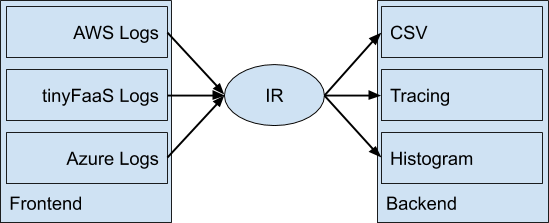
\includegraphics[width=\linewidth,keepaspectratio]{./IR-diagram.png}
\end{center}
\caption[Analysis Architecture Diagram]{%
Analysis Architecture Diagram. 
The frontend part is responsible for aggregating log output from all supported providers
and converting them all into a common format (IR). 
The backend processes can than perform various desired actions on this unified IR data.}%
\label{fig:analysisArchitectureDiagram}
\end{figure}

The analysis tools are split into two main parts. 
The first part (frontend) loads the log files and saves it in a common format, 
whereas the second part (backend) works on this common format and generates e.g.\@ graphs or CSVs
(see \Cref{fig:analysisArchitectureDiagram}).
Thus, the the frontend step only needs to be run once per test run.
Afterwards, we can then repeatedly execute backends against the extracted data.

\section{Frontend}%
\label{sec:analysisFrontend}

The frontend has to parse different log file formats from all supported providers 
which all provide the feature of extracting stdout to their individual logging service. 
The main framework is responsible for downloading those log files in any format and saving them into the local file system. 
The frontend then parses the events from all files into a list of structured events. 
It is important to export and work with the extracted data in various ways which require a different representation of the data. 
Thus, we have decided to introduce an intermediate representation from which each operation can extract their wanted representation. 
The main goal of the frontend is to run an ETL process on the logs and save all events and meaningful data in the IR output file.

\subsubsection{Generic Log Parsing}%
\label{ssub:analysisGenericParsing}

Many providers (such as AWS or Azure) offer a combined structured log format, 
where the functions' stdout stream is inserted into a global provider logs stream. 
Therein, each entry is usually inserted as a JSON object into the provider's stream. 

Since we do not want to write custom programs for each individual platform to extract our actual log statements; 
we have decided to append tokens that are unique to our log messages. 
We can then split the stream into chunks, with each token marking the beginning of a FaasterMetrics lib log statement.
This allows us to use any provider log format, which we don't know ahead of time. 
Assuming no provider chunks or splits stdout streams within their logging, 
and the raw log output is in human-readable text format, 
this approach works universally. 

\begin{figure}
\begin{center}
  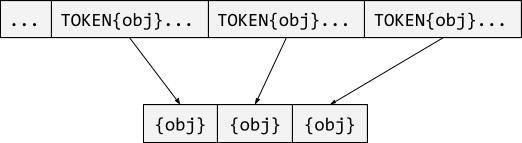
\includegraphics[width=\linewidth, keepaspectratio]{./token-string.png}
\end{center}
\caption[Parsing Log Strings With Tokens]{%
  Depiction of how to extract our library's logging objects out of a generic provider's logging stream.
}
\label{fig:analysisTokenStrings}
\end{figure}

After finding our token separated strings we can easily extract our own event messages, which are in JSON format
(and thus recognizable by their starting and ending brackets).
\Cref{fig:analysisTokenStrings} illustrates this extraction process.

\section{Intermediate Representation}%
\label{sec:analysisIR}

The IR is generated in the frontend and contains all information necessary for the backend processes.
Is has same format for all backends that want to use any of the data generated by the experiments. 
All IR is generated by serializing Python objects into a JSON representation, 
which can be extracted back to Python objects in the backends. 
However, as the common format JSON is used, you can also write programs using our IR in other programming languages.
We provide a comprehensive set of higher-level functions to interact with the IR in python.
These higher-level functions can be found in the Python package \texttt{faastermetrics.helper}.

\section{Backend}%
\label{sec:analysisBackend}

The backend is responsible to load the IR generated by the frontend and convert it to a data structure of choice to produce output from it. 
These backend programs are intended to be written by researchers and end-users who analyse their own experiments. 
We also offer some handy pre-built backend functions, such as a CSV exporter, which translates our IR to CSV.
Details about those provided backend scripts as well as general usage instructions can be found in \Cref{sec:analysisBasicUsage}.

\end{document}
